\subsection{Entity-Relationship Schema}

We decided to start our project starting from the database designed by the e-team group during the FTB course. We report in the following figures the design from we started. In particular in figure \ref{er_original} we reported the ER schema and in Figure \ref{ls_original} the corresponding relational schema.
\newgeometry{top=0.1cm, bottom=0.1cm}
\begin{figure}[H]
\centering
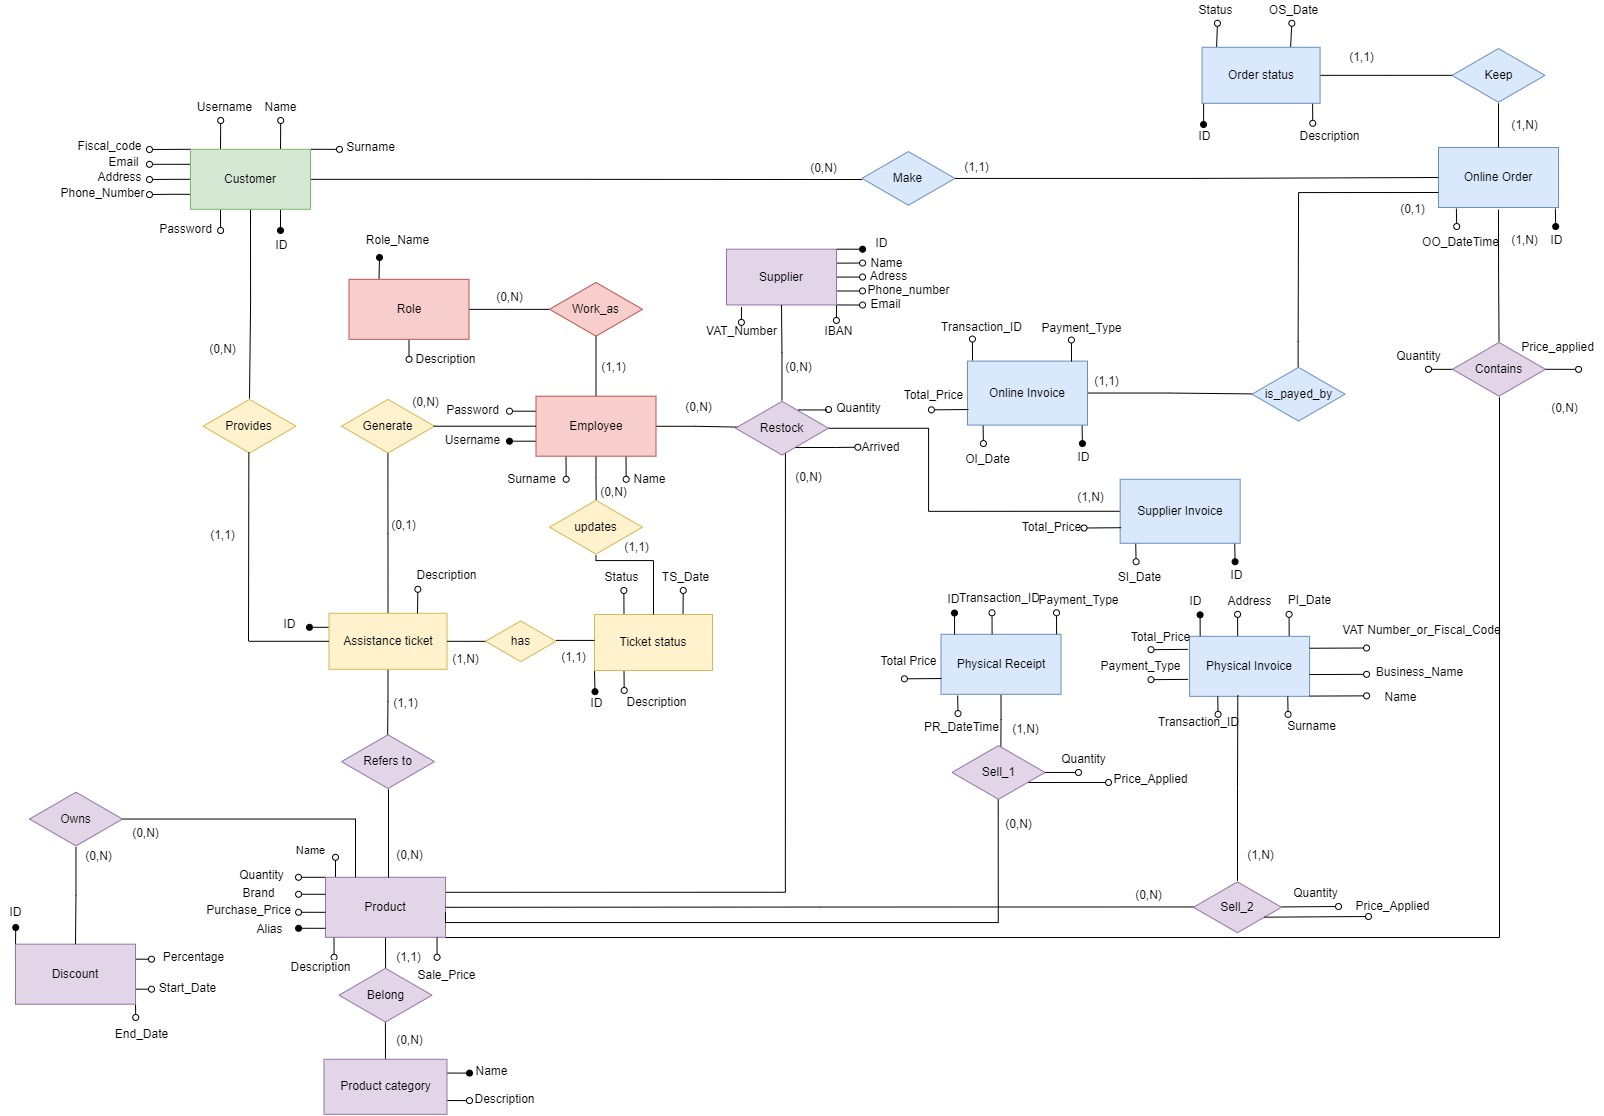
\includegraphics[width=16.5cm]{Schemas/ER_original.jpg}
\caption{Original ER schema designed by e-team}
\label{er_original}
\end{figure}

\begin{figure}[H]
\centering
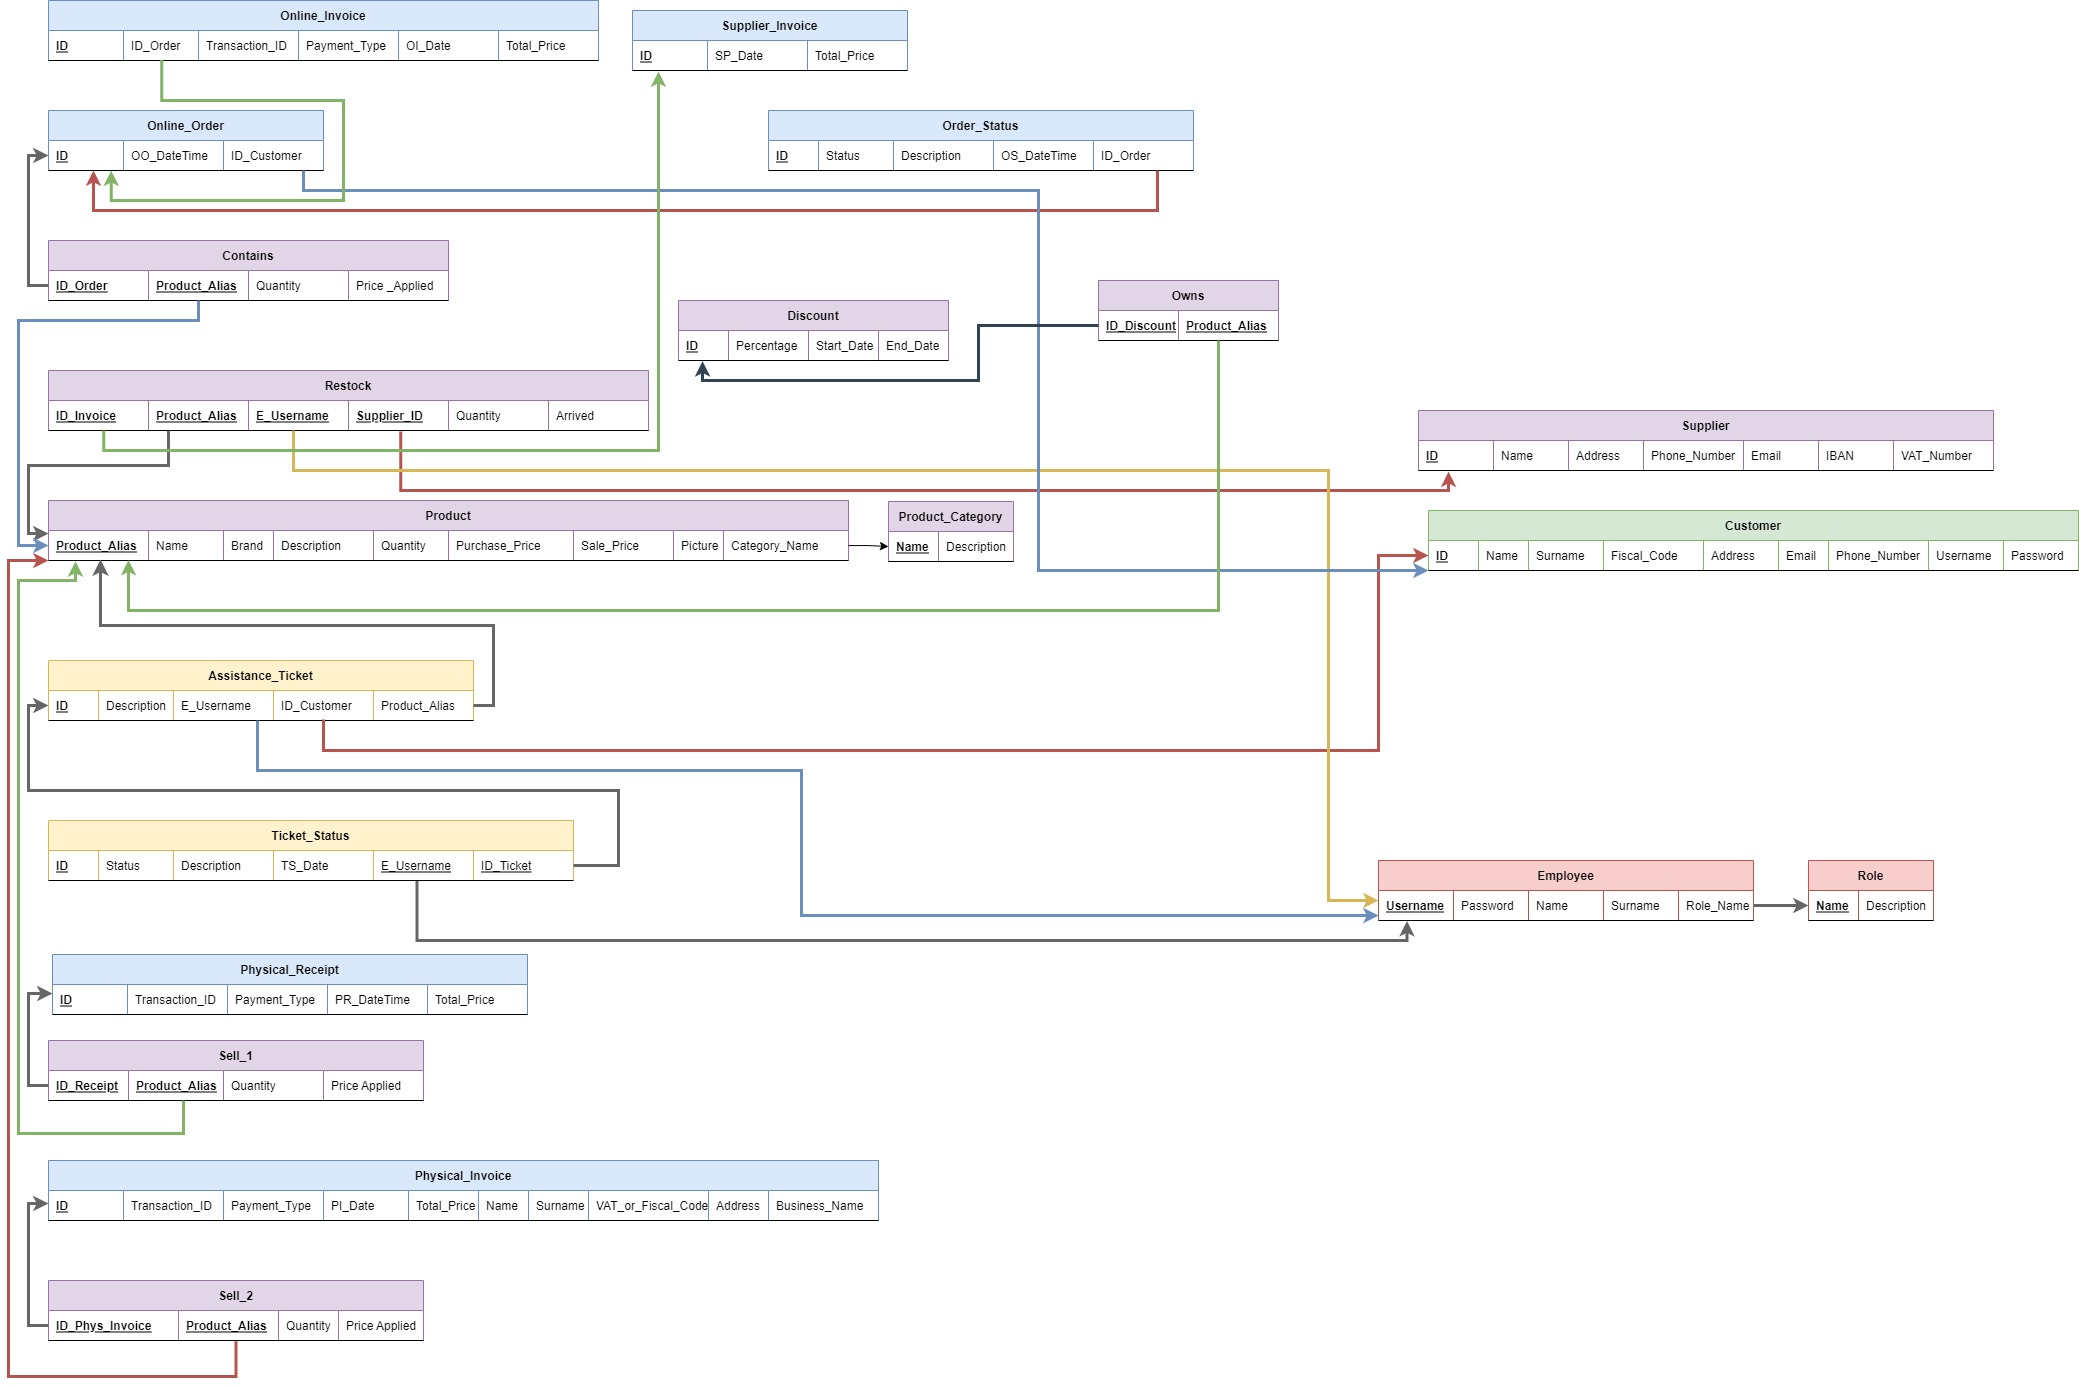
\includegraphics[width=16.5cm]{Schemas/LogicRS_original.jpg}
\caption{Original Relational schema designed by e-team}
\label{ls_original}
\end{figure}
\restoregeometry
In order to maintain the project manageable, we decided to remove some parts. In particular we decided to remove all the "offline services" and to built our web application only to manage the online store.
Another part we removed is the management of the supplier, dedicating the development of our project only to the services seen by the client of the shop (excluding the management of the employees that is need in our web application since we needed them to setting up the permission.). In Figure \ref{er_modified} and \ref{ls_modified} are reported the final version of the design for the data layer(ER schema and relational schema respectively).

\begin{figure}[H]
\centering
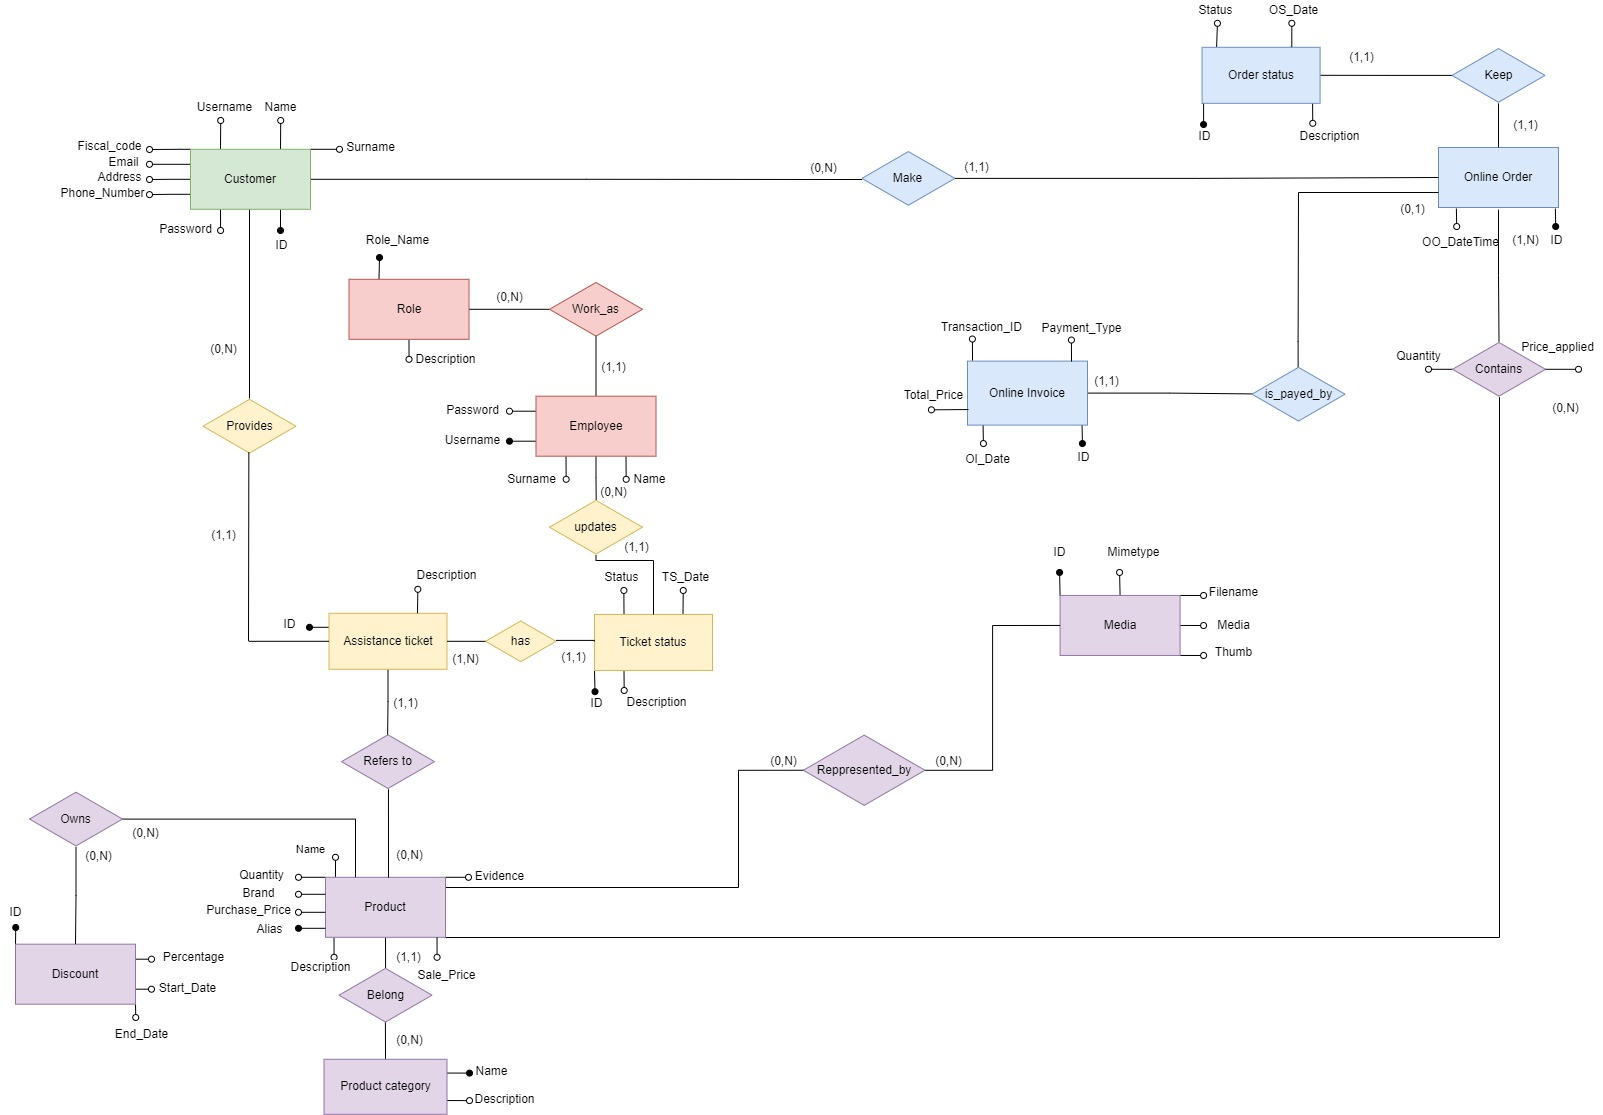
\includegraphics[width=16.5cm]{Schemas/ER_modified.jpg}
\caption{ER schema modified}
\label{er_modified}
\end{figure}

\begin{figure}[H]
\centering
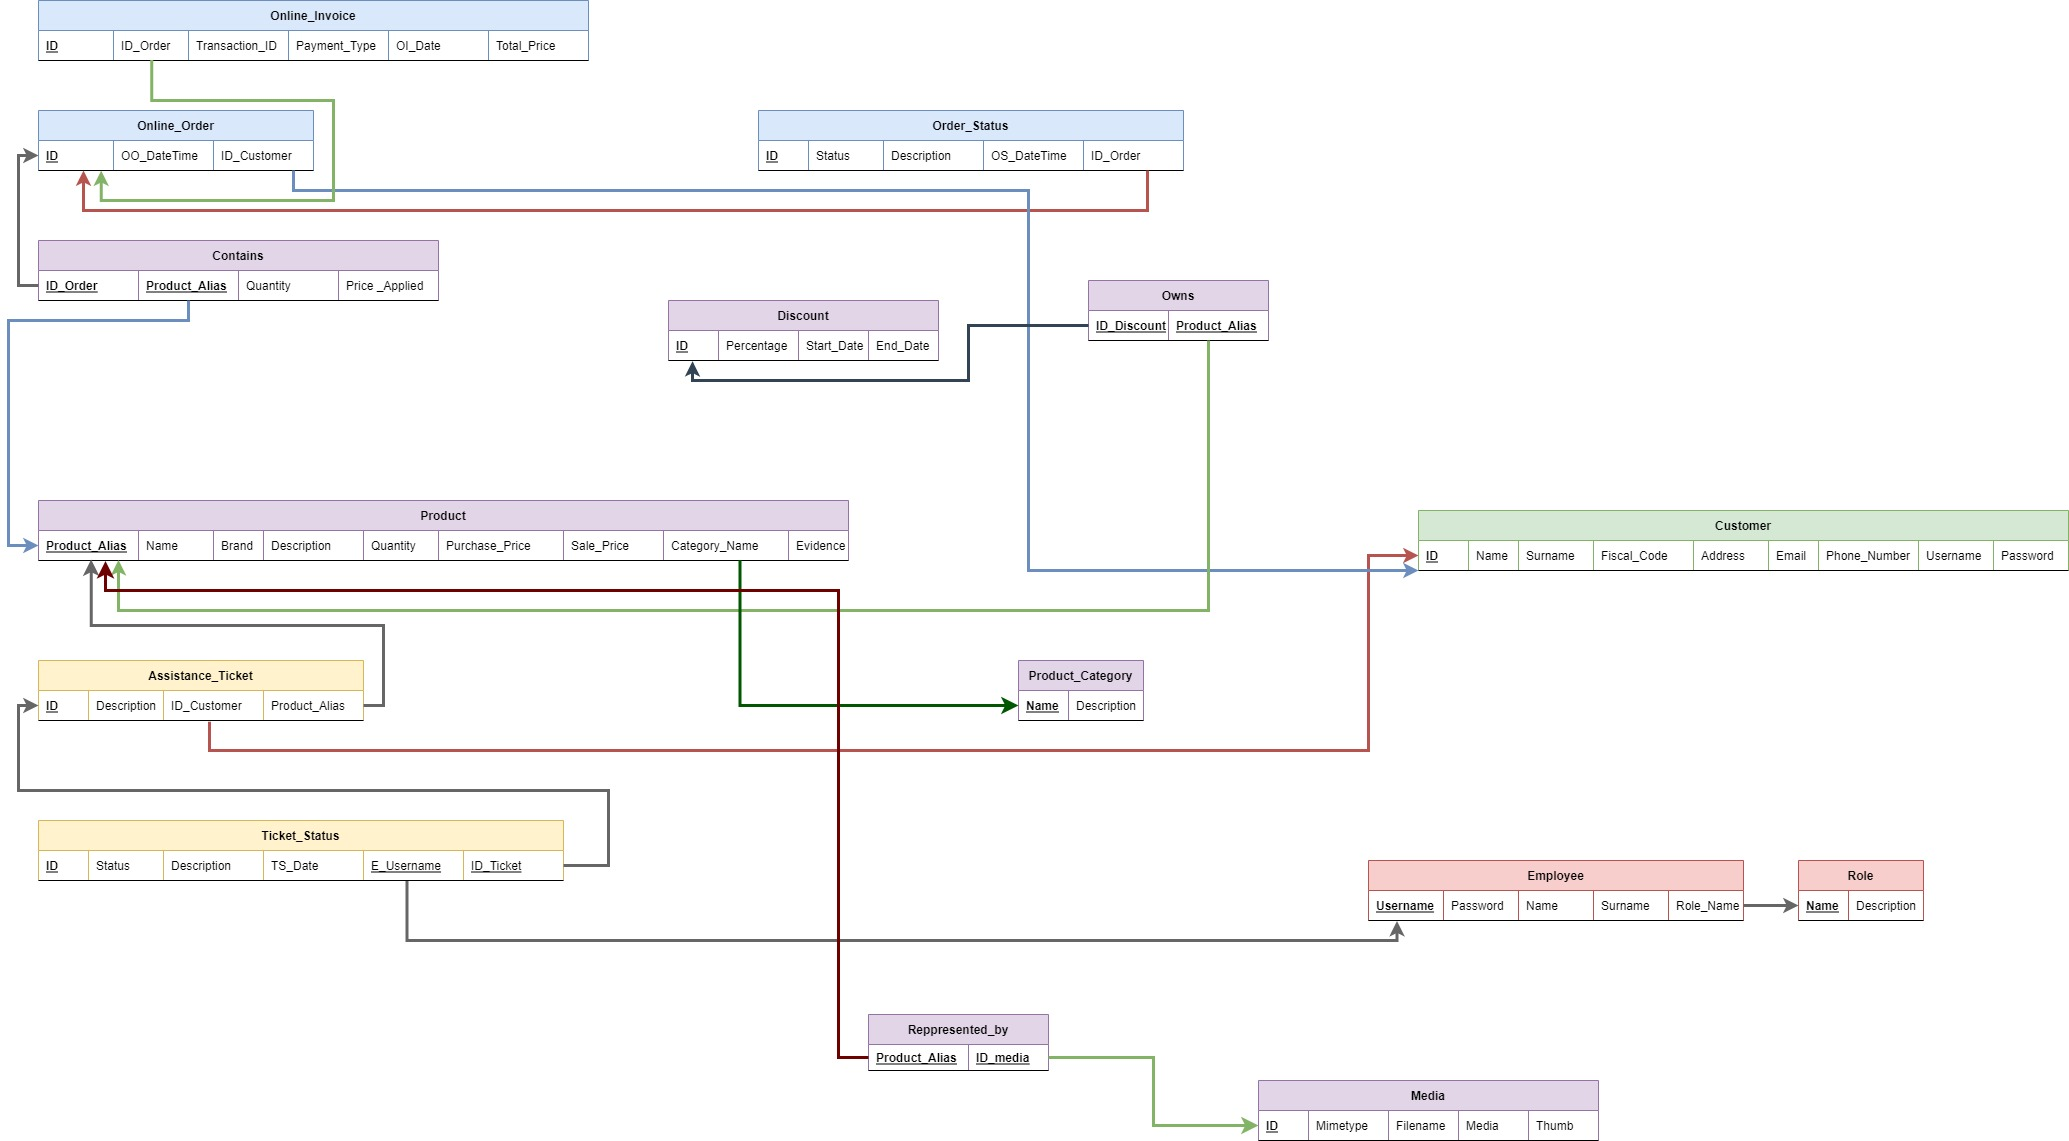
\includegraphics[width=16.5cm]{Schemas/LogicRS_modified.jpg}
\caption{Relational schema modified}
\label{ls_modified}
\end{figure}